\chapter{Schedule and Future Work}
 \label{schedule}
\vspace{-1.9cm}

The detailed timeline of activities is presented in Figure \ref{fig:sched}, which shows the planned progression over each month.

\begin{figure}[ht]
  \centering
  
  % Caption setup for this specific figure
  \captionsetup{
     labelfont={bf,large},       % label (e.g., "Figure 1:") in bold and large
     textfont={bf,large},        % caption text in bold and large
     justification=raggedright,  % left-align the caption
     singlelinecheck=off         % force left alignment even for short captions
  }
  
  \caption{\MakeUppercase{Thesis Schedule}}
  \label{fig:sched}
  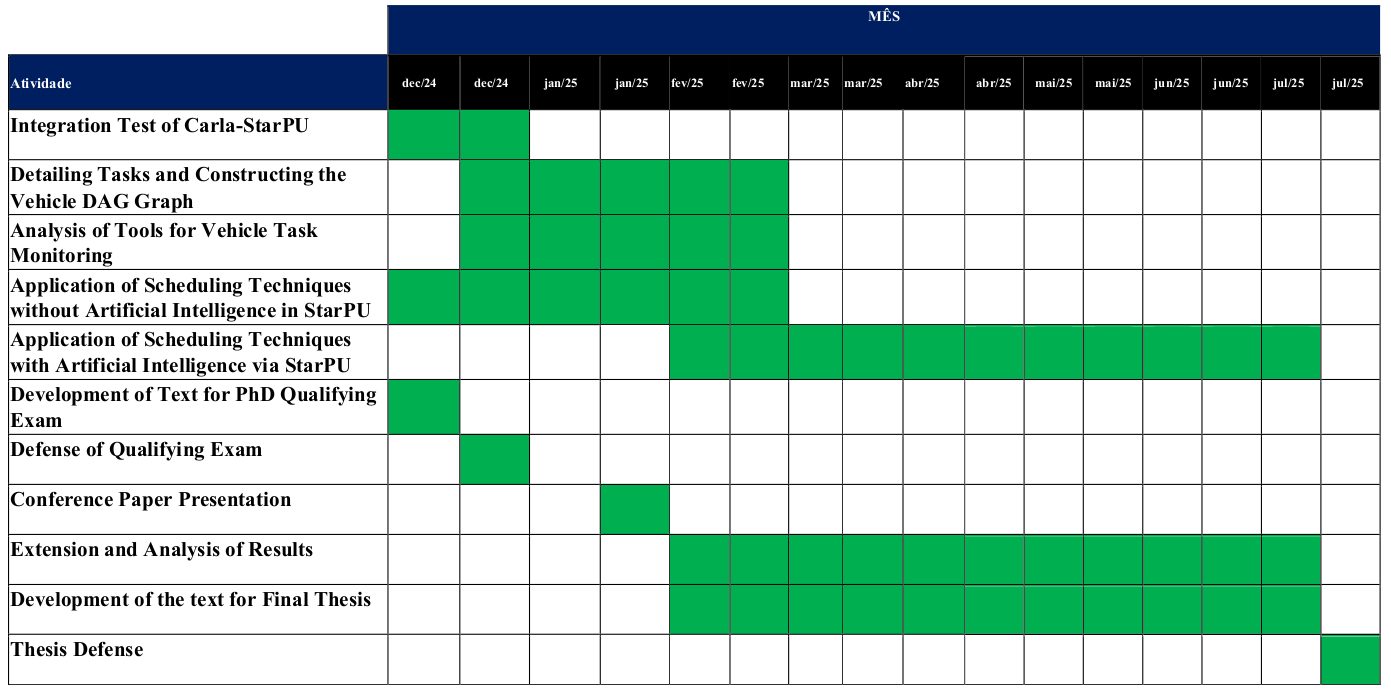
\includegraphics[width=\textwidth, keepaspectratio]{imagens/QualiExt.png}
\captionfont{\small{\textbf{\\Source: Created by the Author}}} 
\end{figure}

The work in progress from Steps 1 to 4 generated the conference paper in Appendix \ref{anexo-accepted} to be present in January 2025. This work is still in progress to consolidate the basic setup using predefined StarPU scheduling strategies. Upon completion of these steps the objective is to start to develop and test the novel scheduling collecting and validating results for the Thesis. The author expects from these results to elaborate one paper submission showing the community the new scheduling method for Autonomous Driving Vehicles. The end of this work is planned to happen by July 2025, however, the intention is to finish the Thesis a couple of months earlier as soon as the development and results are consolidated.
